\section{CAPÍTULO IV: METODOLOGÍA}\label{sec:methodology}

En este capítulo, se describirá la metodología utilizada para conseguir cumplir los objetivos establecidos. 

Se comenzará por discutir el diseño de la investigación y los tipos de variables que serán utilizados a la hora de realizar el estudio. Luego se describirá el enfoque aportado para el preprocesamiento de datos, incluida la limpieza de datos y la selección de características.

Finalmente, se describirán los algoritmos de aprendizaje automático utilizados para el estudio y clasificación de pacientes. 

\subsection{Diseño de Investigación}

Se ha utilizado un enfoque de investigación cuantitativa para examinar la progresión temporal de la bronquiolitis en pacientes pediátricos. Se ha partido de 47 variables descriptivas y de 2 variables que muestran la evolución temporal de los pacientes durante las primeras 24 h de ingreso y que han sido tratadas en el presente trabajo como series temporales. 


Idealmente se ha planteado que al tener 3 momentos de valoración; en las 8 primeras horas, entre las 8 y 16 horas y entre las 16 y 24 horas, se realicen 3 modelos diferentes para los diferentes momentos y que estos modelos permitan valorar la evolución del paciente, es decir si va a necesitar OAF o no va a necesitarla al final de estos intervalos.

En este estudio este planteamiento se muestra limitado puesto que más de la mitad de pacientes que se han considerado válidos para el estudio (según el criterio valid_patient_2 adoptado en el apartado ***) que necesitan OAF la requieren al ingreso o en las primeras 8 horas (De los 16 pacientes válidos que presentan deterioro 10 pacientes; 5 al ingreso y 5 antes de las 8 primeras horas). Esto supondría eliminar de la ecuación estos 10 pacientes y solo tener en cuenta a los 6 restantes para valorar las 8 primeras horas y solo a 2 para valorar las 16 primeras.

\begin{figure}[H]
    \centering
    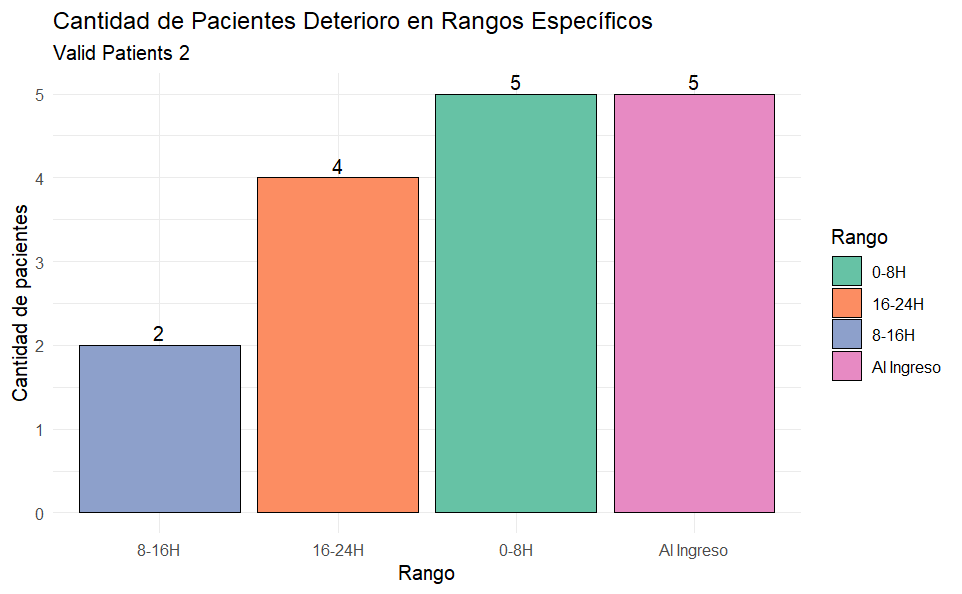
\includegraphics[scale = 1]{./img/bar-deterioro-valid-2.png}
    \caption{Cantidad de Pacientes Deterioro en Rangos Específicos de Tiempo considerando solo los pacientes sgún criterio valid\_patient\_2}
    \label{fig:bar-deterioro-valid-2}
\end{figure}

Se va a separar entre pacientes que han necesitado OAF al ingreso y los que no.

A continuación se muestran en rojo aquellos pacientes que a pesar de haberles suministrado OAF han necesitado ser trasladados a UCIP.

En contraposición se muestran en verde aquellos pacientes que han necesitado OAF pero no han necesitado ser trasladados a UCIP. 



Ningún paciente cómo ya se ha visto ha necesitado traslado a UCIP sin haber necesitado OAF previamente.

